\documentclass{article}

% Language setting
% Replace `english' with e.g. `spanish' to change the document language
\usepackage[english]{babel}

% Set page size and margins
% Replace `letterpaper' with `a4paper' for UK/EU standard size
\usepackage[letterpaper,top=2cm,bottom=2cm,left=3cm,right=3cm,marginparwidth=1.75cm]{geometry}

% Useful packages
\usepackage{amsmath}
\usepackage{graphicx}
\usepackage[colorlinks=true, allcolors=blue]{hyperref}
\usepackage{graphicx}
\graphicspath{ {./images/} }
\usepackage{caption}
\usepackage{subcaption}


\title{Orbits around black holes}
\author{Jordan Moncrieff}

\begin{document}
\maketitle

\begin{abstract}
First task to complete for Honours project.
\end{abstract}

\section{Schwarzschild solution}

\subsection{Task list}

Starting From Schwarzschild metric:

\begin{enumerate}
  \item Calculate gravitational potential for metric - equation (\ref{eq:effective potential schwarzschild}).
  \item Calculate orbits for massive and massless particles - section (\ref{sec:Potential for massive and massless orbits}).
  \item Show innermost stable circular orbit for each and compare them - section (\ref{sec:ISCO})
  \item Make some plots to show how the gravitational potential behaves, and stable orbits in that potential - figure (\ref{fig:Schwarzschild effective potential})
  \item Diagram to show how the location of the ISCO relative to event horizon
  \item Short discussion of implications for an astrophysical black hole - why is having the ISCO different for massive/mass-less particles significant? - section (\ref{sec:Astrophysical significance})
\end{enumerate}

After this, extend to Kerr black hole, explain the differences - section (\ref{sec:Kerr BH}).

Separate the Physics from the maths, what is actually physical?

Look at Perihelion shift, should be very high for Kerr. 

Kerr event horizon is smaller, only relative to an external observer - a observer falling who does not see space-time rapping around in circles will see an event horizon of the Schwarzschild metric. It is just that due to the curvature of spacetime the radius looks smaller.


\section{Governing equations}

\subsection{Einstein's field equations}

We need to solve EFE's, given by 

\begin{equation}
    G_{\mu \nu} + \Lambda g_{\mu \nu} = \kappa T_{\mu \nu}
\label{eq:EFE}
\end{equation}

Where 

\begin{itemize}
    \item $G_{\mu \nu}$ is the Einstein tensor, representing the curvature of space-time.
    
    \item $T_{\mu \nu}$ is the stress energy tensor, representing the density and flux of energy/momentum in space-time.
    
    \item $\Lambda$ is the cosmological constant, representing the expansion of the universe.
    
    \item $\kappa=\frac{8\pi G}{c^4}$ is a constant.
    
    \item $g_{\alpha \beta} = \boldsymbol{e}_\alpha \cdot \boldsymbol{e}_\beta$ is the metric tensor, given by the dot product of the basis vectors, and $g^{\alpha \beta}$ is the inverse metric tensor. The metric tensor allows for measurements of distance in space-time
    .
\end{itemize}

The Einstein tensor can be written as

\begin{equation}
    G_{\mu \nu } = R_{\mu \nu} - \frac{1}{2} R g_{\mu \nu}
\label{eq:Einstein tensor}
\end{equation}

Where the R tensor are contractions of the Ricci tensor defined by equation 

\begin{equation}
    R_{\sigma \mu \nu }^{\rho }=\partial_{\mu} \Gamma _{\nu \sigma }^{\rho }-\partial_\nu \Gamma _{\mu \sigma }^{\rho }+\Gamma _{\nu \sigma }^{\lambda } \Gamma _{\mu \lambda }^{\rho }-\Gamma _{\mu \sigma }^{\lambda } \Gamma _{\nu \lambda }^{\rho }
\label{eq:Riemann tesnor}
\end{equation}


\begin{itemize}
    \item $R_{\mu \nu} = R^{\alpha}_{\nu \alpha \beta}$ is the Ricci curvature tensor, which roughly represents how much the curved space-time deviates from flat space-time.
    \item R = $R^{\alpha}_{\alpha}$ is the Ricci scalar, the contraction of the Ricci tensor, a measure of curvature.
\end{itemize}

And gamma coefficients $\Gamma^{\mu}_{\nu \sigma}$ describes the Christoffel symbols (or affine connection), which itself is given by the formula

\begin{equation}
    \Gamma^{\mu}_{\nu \sigma} = \frac{1}{2} g^{\alpha \mu} (\partial_{\nu}g_{\alpha \sigma}+\partial_{\sigma} g_{\nu \alpha} - \partial_{\alpha} g_{\nu \sigma})
\label{eq:Christoffel symbol}
\end{equation}

Since we are dealing with space-time outside a black hole, assuming a vacuum and covering a distance small enough that expansion of the universe is negligible, we can set $T_{\mu \nu}=0$ (vacuum) and $\Lambda=0$ (ignore expansion). So we are only solving $G_{\mu \nu}=0$. But if we take the trace of equation (\ref{eq:Einstein tensor}), by contracting with inverse metric tensor $g^{\mu \nu}$, we get $R=0$, hence we only need to solve EFE in a vacuum

\begin{equation}
    R_{\mu \nu } = 0
\label{eq:EFE in a vacuum}
\end{equation}

This is 16 coupled non-linear partial differential equations\footnote{The Ricci tensor is symmetric, so it is actually just 10 PDEs.}, involving the calculation of the Christoffel symbols according to equation (\ref{eq:Christoffel symbol}), which themselves depend on the derivatives of the metric components. Due to this high complexity, EFE are only analytically solvable in a few highly symmetric cases, notably the Schwarzschild and the Kerr solutions.

\subsection{Schwarzschild metric}

The distance between two points in space-time is given by the invariant line element $ds^2$. In Schwarzschild space-time, the line is given by equation (\ref{eq:Schwarzschild line-element}) (given in units c=1).

\begin{equation}
    ds^2 = - d\tau^2 = - (1-\frac{2 G M}{r}) dt^2 +  (1-\frac{2 G M}{r})^{-1} dr^2
            + r^2 (d\theta^2+\sin^2\theta d\phi^2)
\label{eq:Schwarzschild line-element}
\end{equation}

I derived the Schwarzschild metric in schwarzschild\_solution.nb, a Mathematica notebook based on the OGRe Mathematica package \cite{Shoshany2021_OGRe} for GR calculations.

\subsection{Kerr metric}

The metric for a Kerr black hole (spherically symmetric, stationary, black hole of mass M rotating at constant angular momentum J) is given by (in units G=c=1)

\begin{equation}\label{eq:Kerr metric}
    ds^2 = -\left(1-\frac{2Mr}{\rho^2}\right) dt^2-\frac{4Mar \sin^2{\theta}}{\rho^2} d\phi dt+ \frac{\rho^2}{\Delta} dr^2 + \rho^2 d\theta^2 +\left(r^2+a^2+
    \frac{2Mra^2\sin^2{\theta}}{\rho^2}
    \right)\sin{\theta}^2 d\phi^2
\end{equation}

Where $a:=\frac{J}{M}$, $\rho^2:=r^2+a^2 \cos{\theta}$, and $\Delta:=r^2-2Mr+a^2$ \cite{carroll2019spacetime}.

It is easy to see that setting $a=0$ leaves us with the Schwarzschild solution (the case of zero spin is the same as Schwarzschild solution in equation (\ref{eq:Schwarzschild line-element})), and in the limit that $r \gg a$ we get the weak field metric (in terms of gravitational potential $\Phi(r)=-\frac{G M}{r}$)

\begin{equation}
    ds^2 = - (1+2\Phi(r)) dt^2 +  (1-2\Phi(r)) dr^2
            + r^2 (d\theta^2+\sin^2\theta d\phi^2)
\label{eq:Weak field metric}
\end{equation}

Which as $r\rightarrow \infty$ approaches flat (Minkowski) spacetime

\begin{equation}
    ds^2 = - dt^2 + dx^2 + dy^2 + dz^2
\label{eq:Minkowski metruc}
\end{equation}



\subsection{Geodesic equation}

The paths followed by particles in general relativity correspond to shortest paths through (curved) space-time. These shortest paths are known as geodesics, and the formula for determining these paths is know as the geodesic equation

\begin{equation}
    \frac{d^2x^{\mu}}{d\tau^2} + \Gamma^{\mu}_{\nu \sigma} \frac{dx^{\nu}}{d\tau} \frac{dx^{\sigma}}{d\tau} = 0
\label{eq:Geodesic equation}
\end{equation}

This equation is derived by minimizing the action $S$ defined by

\newcommand{\Lagr}{\mathcal{L}}

\begin{equation}
    S = \int \mathcal{L}(x_\mu,\dot{x}_\mu) d\lambda = \int \frac{1}{2} g_{\mu \nu} \dot{x}^\mu \dot{x}^\nu d\lambda 
\label{eq:Invariant distance action}
\end{equation}

Using the Euler Lagrange equations

\begin{equation}
    \frac{d}{d\lambda} \frac{\partial \mathcal{L}}{\partial \dot{x_i}} - \frac{\partial \mathcal{L}}{\partial x_i} = 0
\label{eq:Euler-Lagrange equation}
\end{equation}

We can physically motivate this definition by considering that this is equivalent to extremizing the \textit{proper time} $\tau$ between two events\footnote{In special relativity, i.e. flat spacetime, time dilation means that the worldine of free particles moving between two events is the worldline of largest proper time between those events. General relativity says that this principle is extended to curved spacetime.}. The proper time is the time a clock carried by a particle will experience, while a distant observer (at a relative velocity and different gravitational field) will measure a different time between two events. So just find the extremal value of

\begin{equation}
    \tau_{AB} = \int \sqrt{- ds^2} = \int_0^1 \sqrt{-g_{\mu \nu}(x(\lambda))
    \frac{dx^\mu}{d\lambda} \frac{dx^\nu}{d\lambda}}d\lambda 
\label{eq:Proper time}
\end{equation}

Where $\lambda$ is the parametrization of the curve in space. Hence finding the maxima of equation \ref{eq:Proper time} is equivalent to finding the minima of the action given in equation (\ref{eq:Invariant distance action}), as required.

Another way to view equation (\ref{eq:Geodesic equation}) is as a path that is locally straight in curved spacetime. The particles four velocity

\begin{equation}\label{eq:Four velocity}
    \boldsymbol{u} := \frac{dx^\mu}{d\tau}
\end{equation}

Is always tangent to its path in space, the four velocity will therefore be straight if the four vector $\boldsymbol{u}$ does not change after an infinitesimal displacement.

%%%% FININSH GEODESIC EQUATION DERIVATION %%%%
% \begin{alignat}{2}
%     &&\frac{d\boldsymbol{u}}{d\tau} &= 0 \notag\\
%     \Rightarrow
%     &&\frac{d}{d\tau} (u^\mu \boldsymbol{e}_mu) &= 0 \notag\\
%     \Rightarrow
%     &\frac{d}{d\tau} (u^\mu \boldsymbol{e}_=mu) &= 
%     \frac{du^\mu}{d\tau}\boldsymbol{e}_mu + u^\mu \frac{d}{d\tau} u^\mu = 0 \notag\\
%     \Rightarrow
    
% \end{alignat}

% Where the symbol $\Gamma^{\mu}_{\nu \sigma}$ describes the Christoffel symbols (or affine connection), which itself is given by the formula

% \begin{equation}
%     \Gamma^{\mu}_{\nu \sigma} = \frac{1}{2} g^{\alpha \mu} (\partial_{\nu}g_{\alpha \sigma}+\partial_{\sigma} g_{\nu \alpha} - \partial_{\alpha} g_{\nu \sigma})
% \label{eq:Christoffel symbol}
% \end{equation}

\subsection{Effective potential}
Calculating the gravitational potential in general relativity is not as straight forward as it is in Newtonian gravity. There is not a well defined definition for potential in curved spacetime, so instead we define the potential in some region of spacetime to be such that it fits the definition of potential energy that arises from the law of conservation of energy. There are several approaches to be taken, using both the Lagrangian and Hamiltonian definition. I believe the following general procedure, illustrated in later sections, is the following:


\begin{enumerate}
    \item Calculate the Lagrangian defined by equation (\ref{eq:Invariant distance action}).
    \item Use the Euler-Lagrange equation (\ref{eq:Euler-Lagrange equation}) to identify conserved quantities, and equations of motion for geodesic.
    \item Use conserved quantities, along with the identity in equation (\ref{eq:Metric constant}) - which depends on weather you are interested in massive or massless orbits - to simplify the Lagrangian in terms of conserved quantities.
    \item Rewrite the Lagrangian equation to clearly identify the effective kinetic energy ($\frac{1}{2} \left( \frac{dr}{d\tau} \right)^2$), the effective total energy (some function of the conserved quantity E), and the effective potential energy (whatever remains).
\end{enumerate}  

\subsection{Event horizon}\label{sec:Event horizons}

The event horizon of a black hole is an imaginary boundary in space surrounding a black hole, such that anything (including light) within that boundary will be unable to escape the black hole, so the future of that particle is the singularity at the origin (r=0) of the black hole. In the Schwarzschild solution, the event horizon coincides with the point where a photon experiences infinite time-dilation, and hence infinite redshift according to an observer at infinity. Hence, the event horizon occurs when $g_{tt}=0$, from equation (\ref{eq:Schwarzschild line-element}) this occurs when $1-\frac{2GM}{r}=0$, i.e. the Schwarzschild radius is $r=\frac{2GM}{r}$.

The problem of finding the event horizon is more complicated in less idealized black holes, such as in the Kerr metric, where a photon can pass the surface of infinite redshift, and still return to a larger radius. The surface between the event horizon and the infinite redshift surface is known as the \textit{ergoregion}. The surface of infinite redshift can be found by setting $g_{tt}=0$, so from equation (\ref{eq:Kerr metric}) we find 

\begin{alignat}{2}
    &&1-\frac{2 M r}{r^2+a^2 \cos{\theta}} &= 0 \notag \\
    \Rightarrow
    && 2 M r &= r^2 - a^2 \cos{\theta} \notag \\
    \Rightarrow
    &&r_{\pm} &= M \pm \sqrt{M^2+a^2 \cos{\theta}}\label{eq:Kerr infinite redshift radius}
\end{alignat}

The event horizon can be found by finding when $g_{rr}$ diverges in equation (\ref{eq:Kerr metric}), i.e. when $\Delta = 0$, giving the event horizon radius

\begin{equation}
    r_{\rm{eh,}\pm} = M \pm \sqrt{M^2 - a^2}
\end{equation}\label{eq:Kerr event horizon radius}

So we can see the two regions overlap at the poles (as expected, since there is locally no difference to a Schwarzschild black hole at region where there is no rotation), but the sphere of infinite redshift extends further in all other regions. The region between these two surfaces is called the \textit{ergosphere}.

Note that particles can escape a Kerr black hole near its equator relatively easily compared to a Schwarzschild black hole, i.e. the event horizon is somehow "squished" along the equator due to the black holes spin. The reason for this is that Kerr event horizon is smaller, only relative to an external observer - a observer falling who does not see space-time rapping around in circles will see an event horizon of the Schwarzschild metric. It is just that due to the curvature of spacetime the radius looks smaller.


% Make warning sign
\newcommand\Warning{%
 \makebox[1.4em][c]{%
 \makebox[0pt][c]{\raisebox{.1em}{\small!}}%
 \makebox[0pt][c]{\color{red}\Large$\bigtriangleup$}}}%

\newunicodechar{⚠}{\Warning} Is this legit


Can also intuitively think of as the result of frame dragging, where particles around Kerr black hole begin rotating about the black hole in line with the rotation. This gives the particles extra angular momentum, increasing the effective potential of the particle, meaning it takes less energy for the particle to escape. Can also think of a centrifugal force term contributing to the escape.



\subsection{Constants of motion}
Solving the Geodesic equation directly would be extremely difficult, if not impossible. Calculations in GR almost always require the use of constants of motion in order to be able to solve even the simplest problems.

We will exploit what is essentially conservation of energy and conservation of angular momentum.

Plugging in $\mu=t$ into equation (\ref{eq:Geodesic equation}), using equation (\ref{eq:Christoffel symbol}) to calculate the required Christoffel symbols, we can show that the following quantity (corresponding to the energy per unit mass of a test particle at infinity) is conserved

\begin{equation}
    E = (1-\frac{2 G M}{r}) \frac{dt}{d\tau}
\label{eq:Energy conservation}
\end{equation}

This energy symmetry is a result of time symmetry, specifically the invariance of the metric with respect to time $\partial_t g_{\mu \nu} = 0$\footnote{This is a result of Noether's theorem, symmetries result in conserved quantities.}. So this symmetry won't exist in more general space-time (it will in Kerr and static Schwarzschild spacetimes, but not for binary orbits).

Another conserved quantity can be found\footnote{These conserved quantities will also pop out of the Euler Lagrange equations applied to the Lagrangian described earlier.} by substituting $x=\phi$ into equation (\ref{eq:Geodesic equation}), yielding the conserved quantity

\begin{equation}
    r^2 \sin^2\theta \frac{d\phi}{d\tau} = L
\end{equation}

Corresponding to the angular momentum per unit mass (if observed at infinity). This corresponds to rotational symmetry (won't exist in binary orbit).

The final symmetry to solve the geodesic equation comes from the quantity

\begin{equation}
    d\tau^2 = - g_{\mu \nu} dx^{\mu} dx^{\nu}\implies
    % 1 = - g_{\mu \nu} \frac{dx^{\mu}}{d\tau} \frac{dx^{\nu}}{d\tau}
    - g_{\mu \nu} \frac{dx^{\mu}}{d\tau} \frac{dx^{\nu}}{d\tau} = 
    \begin{cases}
        1,& \text{if } d\tau > 0\\
        0,              & \text{if } d\tau = 0
    \end{cases}
\end{equation}
But this is just conservation of (four) momentum $P^\mu:=m \frac{dx^\mu}{d\tau}$. Indeed the contraction $P_\mu P^\mu $ is a scalar, so it must be the same in all inertial reference frames. Hence by considering a particle at $r=\infty$ in a frame such that the particle is at rest, we see all velocity components are zero, leaving the only non-zero component to be $P^0=m \frac{dt}{d\tau}=m$, we can see $P_\mu P^\mu = \eta_{\mu \nu} P^\mu P^\nu = -m^2$ for non-zero mass. Since this is a scalar quantity, it will be the same in all reference frames, and will be a constant. Hence we get the conservation of four momentum to be

\begin{alignat}{2}
    &&g_{\mu \nu} P^\mu P^\nu &= -m^2 \\
    &\Rightarrow
    &g_{\mu \nu} m \frac{dx^\mu}{d\tau} m \frac{dx^\nu}{d\tau} &= -m^2 \notgag \\
    &\Rightarrow
    & g_{\mu \nu}  \frac{dx^\mu}{d\tau}  \frac{dx^\nu}{d\tau} &= -1 \notgag
\end{alignat}

Which implies equation (\ref{eq:sigma conservation}) for the case of massive particles, and similar reasoning can be used to justify the $d\tau=0$ case.

\begin{alignat}
    P^\mu = m \frac{dx^\mu}{d\tau}
    
\end{alignat}

\label{eq:Metric constant}
\end{equation}

\newunicodechar{⚠}{\Warning} \newunicodechar{⚠}{\Warning}Explain the physical meaning of this conservation.

Since we have two different situations for massive ($d\tau >0$) and massless ($d\tau=0$, e.g. photons) particles, so we can rewrite equation (\ref{eq:Metric constant}) as $- g_{\mu \nu} dx^{\mu} dx^{\nu} = \sigma$, where $\sigma = 0$ for massless particles, and $\sigma = 1$ for massive particles.

This gives us the formula

\begin{equation}
    -\sigma = - (1-\frac{2 G M}{r}) (\frac{dt}{d\tau})^2 +  (1-\frac{2 G M}{r})^{-1} (\frac{dt}{dr})^2
            + r^2 ((\frac{d\theta}{dt})^2+\sin^2\theta (\frac{d\phi}{dt})^2)
\label{eq:sigma conservation}
\end{equation}


Using equation (\ref{eq:sigma conservation}), along with conservation of energy and angular momentum to eliminate $\frac{dt}{d\tau}$ and $\frac{d\phi}{d\tau}$, and impose $\theta=\pi / 2$ (which we can do without loss of generality, due to spherical symmetry and the fact that orbits in Schwarzschild space-time lie in a fixed plane) we can arrive at

\begin{equation}
    \frac{1}{2} \left(\frac{dr}{d\tau}\right)^2
    + V\left(r\right) = \frac{1}{2} E^2
\label{eq:conservation of E Schwarzschild}
\end{equation}

Where we have defined the effective potential energy

\begin{equation}
    V\left(r\right) := \frac{1}{2} \sigma - \sigma \frac{G M}{r} + \frac{L^2}{2 r^2} - \frac{G M L^2}{r^3}
\label{eq:effective potential schwarzschild}
\end{equation}

So we can plot the effective potential for different $L/M$ ratios.

\begin{figure}[h]
    \centering
    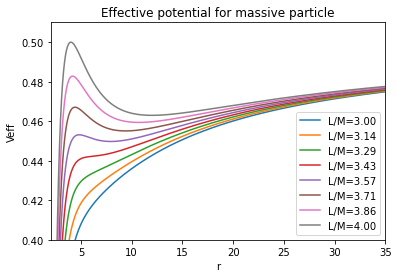
\includegraphics[width=7cm, height=8cm]{images/massive_particle_S.png}
    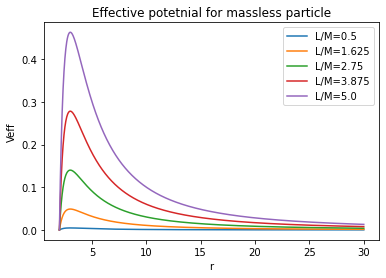
\includegraphics[width=7cm, height=8cm]{images/massless_particle_S.png}
    \caption{Schwarzschild effective potential, varying angular momentum to mass ratio. Note the Schwarzschild radius is a constant $r_s=2 G M$, and since we have set $G M = 1$ in this diagram, this corresponds to the point $r=2$ - can see the potential is zero at the event horizon.}
    \label{fig:Schwarzschild effective potential}
\end{figure}

\subsection{Potential for massive and massless orbits}\label{sec:Potential for massive and massless orbits}

A circular orbit will occur at the point where the derivative of the effective potential is zero. If these potential correspond to a maxima, they are unstable, if it corresponds to a minima, it is stable. Looking at figure (\ref{fig:Schwarzschild effective potential}) we can immediately see the mass-less particles only form unstable circular orbits, with the radius increasing with the L/M ratio.

Massive particles, as seen in the diagram, there are either zero circular orbits, or one stable and one unstable circular orbit (when L/M ratio gets high enough). It is easy to prove all of this by differentiating equation (\ref{eq:effective potential schwarzschild}) with respect to r, and solving the equation for r.

\begin{alignat}{2}
    &&V'(r)&=0\notag\\
    &\Rightarrow\quad
    &\frac{\sigma G M}{r^2} - \frac{L^2}{r^3} + \frac{3 G M L^2}{r^4}
    &=0 \label{eq:derivative=0}\\
    &\Rightarrow\quad 
    &r_{c,\pm}
    &=\frac{L^2 \pm \sqrt{L^4-12 \sigma G^2 M^2 L^2}}{2 \sigma G M}\label{eq:r+-}
\end{alignat}

\subsection{ISCO}\label{sec:ISCO}

So there exists solutions to this equation for $\sigma=1$ (massive particles) if the value inside the square root of equation (\ref{eq:derivative=0}) is non-negative, i.e. $L^2 < 12 (G M)^2$. We can see geometrically from the plots that for such solutions, the negative corresponds to the unstable circular orbit, while the positive corresponds to the outer stable orbit. These two orbits appear when $L=2\sqrt{3}GM \Rightarrow\quad r_{c,+}=r_{c,-}=6(GM)$\footnote{$r_c=6 GM$ is the "inner-most stable circular orbit.}, and in the limit as $L\longrightarrow \infty$ is $r_{c,-}=0$ from (\ref{eq:r+-}), and equation (\ref{eq:derivative=0}) implies that $r_{c,+}\rightarrow GM$. Since the inner orbit is unstable, any perturbation will radially inward will cause the particle to spiral into the event horizon at $r=2GM$, and any perturbation radially outward will cause the particle to move to the stable outer orbit. 

Hence, massive particles have stable circular orbits for 

\begin{equation}
    6 G M \leq r \leq \infty \iff 2\sqrt{3} \leq \frac{L}{M} \leq \infty
\end{equation}

\subsection{Massless particle}

The mass-less orbits can be found by setting $\sigma=0$, so from equation (\ref{eq:derivative=0}) we immediately see that there is only one solution, $r_c=3GM$, independent of any other factor. We also see graphically, that it is an unstable orbit (it corresponds to a maxima, could do second derivative test). It should be mentioned that mass-less particles do not have a well defined angular momentum L, L is only a physical value when the ratio $\frac{L}{E}$ is taken. 

$\frac{L}{E} = 3\sqrt{3}GM$ is critical value, the impact parameter shows whether the light ray is absorbed by black hole. This can be seen by noting that a particle is bound to an orbit if $E \leq V_{\rm{eff}}$, since $V_{\rm{eff}}(r_c=3GM) \gt \frac{E^2}{2} \Rightarrow \frac{E^2}{2} \lt \frac{L^2}{54GM}$.

The reason that there is no \textit{stable} circular orbit for light rays is that light travels in a straight path, and since the curvature towards the BH will be monotonically increasing towards the black hole, any perturbation outward/inward from a circular orbit will result in the photon continuing out from the straight line orbit around the black hole. Massive particles have some additional properties that make them behave differently, namely their mass and angular momentum. 

% I would guess the same is not true of particles with mass, as they have mass that contributes to the curvature of space within its neighbourhood of spacetime, so there could be an effect where the particle rolls back into its stable orbit after a small perturbation, due to its self gravity.

Shapiro delay

\subsection{Particle orbits}

Equation \ref{eq:conservation of E Schwarzschild}, we have

\begin{equation}
    \left (\frac{dr}{d\tau} \right )^2 = E^2 - \sigma \left( 1 - 2 \frac{G M}{r} \right) - \frac{L^2}{2 r^2} - \frac{G M L^2}{r^3}
\end{equation}

Can manipulate this into a second order DE to give radius as a function of angle phi. This is not exactly solvable, but we can either expand as a perturbation of the exactly solvable Newtonian case (conic sections), or solve numerically for given boundary conditions.

\begin{figure}
    \centering
    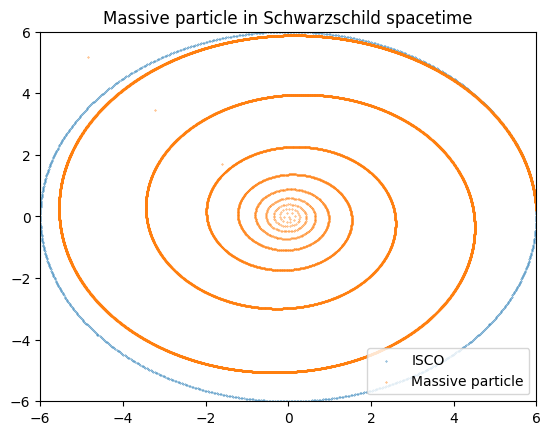
\includegraphics[width=0.5\textwidth]{images/shitty_orbit_program.png}
    \caption{Terrible orbit program. Make a better one}
    \label{fig:terrible orbit program}
\end{figure}


\begin{figure}
    \centering
    \includegraphics[width=0.66
\textwidth]{images/schwarzschild_orbits.png}
    \caption{Diagram showing difference between massive and massless particle orbits in Schwarzschild spacetime. Can see the Photon orbit is close to the black hole, and is unstable. These orbits can be compared to the event horizon}
    \label{fig:Scwarzschild orbits}
\end{figure}

\begin{figure}
    \centering
    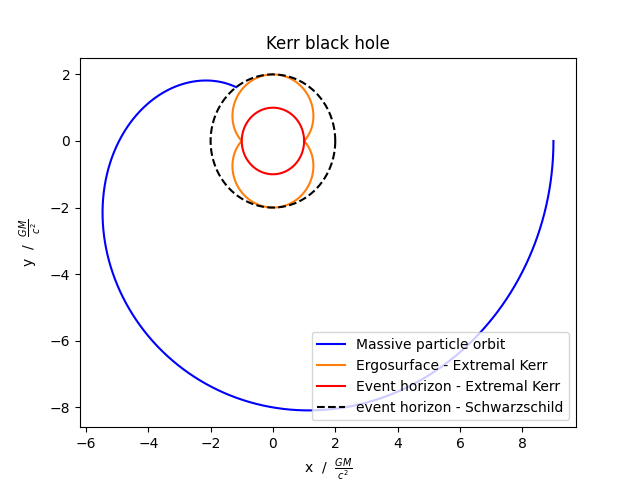
\includegraphics[width=0.66\textwidth]{images/Kerr_orbits.png}
    \caption{Kerr massive particle circular orbit for extremal black hole (a=1). It does not work, don't know why.}
    \label{fig:Kerr massive particle orbit}
\end{figure}


\begin{figure}[h]
     \centering
     \begin{subfigure}[b]{0.3\textwidth}
         \centering
         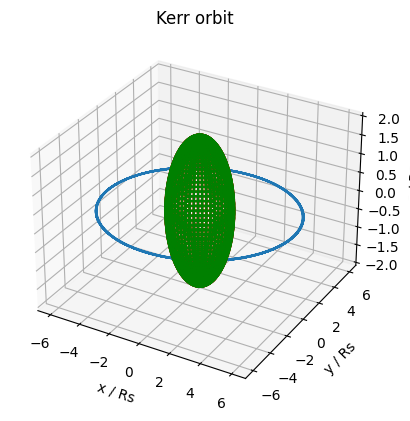
\includegraphics[width=\textwidth]{images/kerr_a=0_del.png}
         \caption{a=0.0}
         \label{fig:Kerr orbit, a=0}
     \end{subfigure}
     \hfill
     \begin{subfigure}[b]{0.3\textwidth}
         \centering
         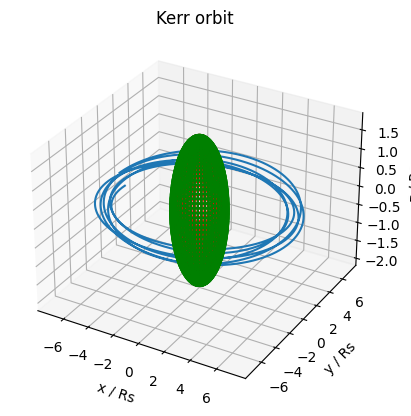
\includegraphics[width=\textwidth]{images/kerr_a=0.5.png}
         \caption{a=0.5}
         \label{fig:Kerr orbit, a=0.5}
     \end{subfigure}
     \hfill
     \begin{subfigure}[b]{0.3\textwidth}
         \centering
         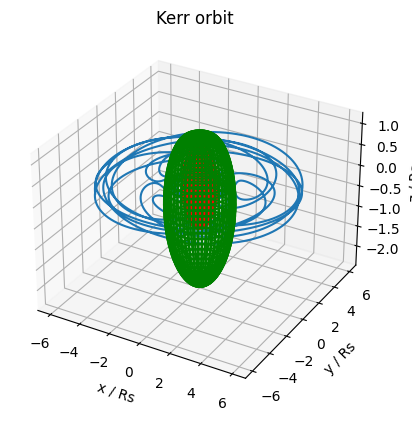
\includegraphics[width=\textwidth]{images/kerr_a=1.png}
         \caption{a=1.0}
         \label{fig:Kerr orbit, a=1.0}
     \end{subfigure}
        \caption{Effect on orbits as spin increases}
        \label{fig:Effect of spin on orbit}
\end{figure}


\section{Kerr black hole}\label{sec:Kerr BH}

\subsection{Form of the metric}

The general form of a space-time metric is

\begin{alignat}{1}
    ds^2&=g_{\mu \nu} dx^{\mu} dx^{\nu}\notag\\
    &=g_{tt}(t,x^i) dt^2 + 2 g_{ti}(t, x^i) dx^t dx^i + g_{ij}(t, x^i) dx^i dx^j
\label{eq:general form of metric}
\end{alignat}

Where the Greek indices $\mu, \nu = 0,1,2,3$ run over both time and space indices (we are using spherical polar coordinates, so $(x^0,x^1,x^2,x^3)=(t,r,\theta,\phi)$), while Latin indices $i, j = 1,2,3$ run only over spatial indices. We now go through the procedure to find the symmetries of the system such that the metric takes the simplest form, giving us a chance to solve the Einstein field equations (EFE) analytically. Note the following symmetries




\begin{enumerate}
    \item Time translation $t \rightarrow t-a\Rightarrow g_{\mu \nu}(t,x^i)=g_{\mu \nu}(x^i)$.
    
    \item \newunicodechar{⚠}{\Warning} Time reversal $t \rightarrow -t$.
    
    \item Axial symmetry $\phi \rightarrow \phi + a\Rightarrow g_{\mu \nu}(x^i)=g_{\mu \nu} (r, \theta)$.

    \item $\theta \rightarrow -\theta \Rightarrow$ cross terms involving $\theta$ are zero.
\end{enumerate}

The metric tensor transforms as any (2,0) tensor, i.e. for a coordinate transform $x^{\alpha} \rightarrow x^{\alpha'}$, the metric transforms $g_{\mu \nu} \rightarrow g'_{\mu \nu}$ according to the transformation law

\begin{equation}
    g'_{\mu \nu} = \frac{\partial x^{\alpha}}{\partial x^{\mu'}} \frac{\partial x^{\beta}}{\partial x^{\nu'}} g_{\alpha \beta}
\label{eq:metric transformation}
\end{equation}


Time reversal symmetry, \textbf{which we do not have for a Kerr black hole}, would mean that $g_{\mu \nu}(t, x^i) = g'_{\mu \nu}(t, x^i)$ for a coordinate transformation $t=x^0 \rightarrow x^{0'}=-t$. So plugging this into equation (\ref{eq:metric transformation}) we get 

\begin{alignat}{2}
    &&\frac{\partial x^0}{\partial x^{0'}} &= -1 \notag \\
    &&\frac{\partial x^i}{\partial x^{i'}} &= +1 \notag \\
    &\Rightarrow
    &g'_{\mu \nu} &= \frac{\partial x^{\alpha}}{\partial x^{\mu'}} \frac{\partial x^{\beta}}{\partial x^{\nu'}} g_{\alpha \beta}\notag \\
    &\Rightarrow
    &g'_{\mu t} &= \frac{\partial x^{\alpha}}{\partial x^{\mu'}} \frac{\partial x^{\beta}}{\partial x^{t'}} g_{\alpha \beta}\notag \\
    &&&=\frac{\partial x^{\alpha}}{\partial x^{\mu'}} \left( -1 \right) g_{\alpha t}\notag \\
    &&&=-g_{\mu t}
\end{alignat}

But, $g_{\mu t} = g'_{\mu t}$, hence $g_{\mu t}=0, \forall \mu \neq t$. This is what eliminated the cross terms in the Schwarzschild metric, but in the Kerr metric there is still the cross term $d\phi dt$, since space-time is different for objects rotating with the spin of the black hole, and objects orbiting in opposite direction to the black hole (frame dragging). However, cross terms like $dr dt$ must be zero, because stepping outward a radial distance in forward time dt should be an equivalent distance to stepping inward dr at negative time -dt. 


\subsection{Symmetries}

To go through the same procedure to find particle orbits as we did for the Schwarzschild solution, we need to go through the same step of finding integrals of motion. We will approach this slightly more rigorously in our second attempt, by introducing the concept of \textit{Killing vectors}. See the appendix.

The Kerr solution is stationary (does not depend on time), hence $(t,r,\theta,\phi)\rightarrow(t+a,r,\theta,\phi)$ is a symmetry, corresponding to the Killing vector with components $\xi^{\alpha}=(1,0,0,0)$. The solution is also independent of $\phi$ since $(t,r,\theta,\phi)\rightarrow(t+a,r,\theta,\phi)$ has no effect on the system, hence another Killing components is $\eta^{\alpha}=(0,0,0,1)$. These correspond to Killing vectors 

% \begin{alignat*}{1}
%     \textbf{\xi}&=\xi^{\alpha}\partial_{\mu}=\partial_t
%     \textbf{\eta}&=\eta^{\alpha}\partial_{\alpha}=\partial_{\phi}
% \end{alignat*}

\begin{alignat}{2}
    \boldsymbol{\xi}&=\xi^{\alpha}\partial_{\mu}=\partial_t\notag\\
    \boldsymbol{\eta}&=\eta^{\alpha}\partial_{\alpha}=\partial_{\phi}\notag
\end{alignat}

Killing vectors give us conserved quantities according to 

\begin{equation}
    \boldsymbol{K_\mu} \frac{dx^\mu}{d\tau} = const.
\end{equation}

So when $p^\mu=m\frac{dx^\mu}{d\tau}$ we also have $\boldsymbol{K_\mu} p^\mu = const.$ as well. So for $\boldsymbol{K}=\boldsymbol{\eta}$ we get 

\begin{alignat}{2}
    e  &= -g_{\mu \nu} \xi^{\mu} u^{\nu} \notag \\
       &= -g_{00}  \xi^0 u^0 - g_{03} \xi^0 u^3 \notag \\
       &= \left(1-\frac{2Mr}{\rho^2}\right) \frac{dt}{d\tau} + \left( \frac{4Mr A^2 \sin^2{\theta}}{\rho^2} \right)\frac{d\phi}{d\tau}  \label{eq:energy conserve Kerr} \\
    l &=g_{\mu \nu} \eta^{\mu} u^{\nu} \notag \\
      &= g_{30}  \eta^3 u^0 + g_{33} \eta^3 u^3 \notag \\
      &= - \left(\frac{4Mr A^2 \sin^2{\theta}}{\rho^2} \right) \frac{dt}{d\tau} + \left( r^2+a^2+\frac{2 M r a^2 \sin^2{\theta}}{\rho^2} \right) \frac{d\phi}{d\tau}
      \label{eq:angular momentum conserve Kerr}
\end{alignat}

Combining equations (\ref{eq:energy conserve Kerr}) and (\ref{eq:angular momentum conserve Kerr}) we can solve for $\frac{d\phi}{d\tau}$ and $\frac{dt}{d\tau}$.

\begin{equation}
    \frac{dt}{d\tau} =
        \frac{1}{\Delta}\left[(r^2+a^2+\frac{2 M a^2}{r}) e - \frac{2 M a}{r} l \right] \\
\end{equation}\label{eq:Kerr dtdtau}
\begin{equation}
    \frac{d\phi}{d\tau} =
        \frac{1}{\Delta} \left[ \left( 1-\frac{2 M}{r}
 \right) l+\frac{2 M a}{r} e \right]
\end{equation}\label{eq:Kerr dphidtau}

Then plugging these into the relation from equation (\ref{eq:Metric constant}), and (for now) assuming a equatorial orbit (so that we can set $\frac{d
\theta}{d\tau}=0$), we arrive at the equation for a massive particle

\begin{alignat}{2}
    \frac{e^2-1}{2} &= \frac{1}{2} \left(\frac{dt}{d\tau} \right)^2 + V_{\rm{eff}} (r, e, l) \\
    V_{\rm{eff}} (r, e, l) &:= - \frac{M}{r} + \frac{l^2 - a^2 (e^2-1)}{2 r^2} - M \frac{(l - a e)^2}{r^3}
\end{alignat}

As well as for a massless particle, which must be parameterised by a different parameter, $\lambda$, since massless particles have constant proper time $\tau$

\begin{alignat}{2}
    \frac{1}{l^2} \left( \frac{dr}{d\lambda} \right)^2 &= \frac{1}{b^2} - W_{\rm{eff}} (r, b, l) \\
    W_{\rm{eff}} (r, b, l) &:= \frac{1}{b^2} - \frac{1}{r^2} \left[  1-\frac{a^2}{b^2} -\frac{2M}{r} \left(  1-\rm{sign}(l) \frac{a}{b}   \right)^2  \right]
\end{alignat}

$p^0=E$ a constant (conservation of energy), and for $\boldsymbol{K}=\boldsymbol{\xi}$ we get $p^3=m \frac{d\phi}{d\tau}=L$ a constant (conservation of angular momentum)


% $\textbf{\xi}=\xi^{\alpha}\partial_{\mu}=\partial_t$ and $\textbf{\eta}=\eta^{\alpha}\partial_{\alpha}=\partial_{\phi}$

\begin{figure}
    \centering
    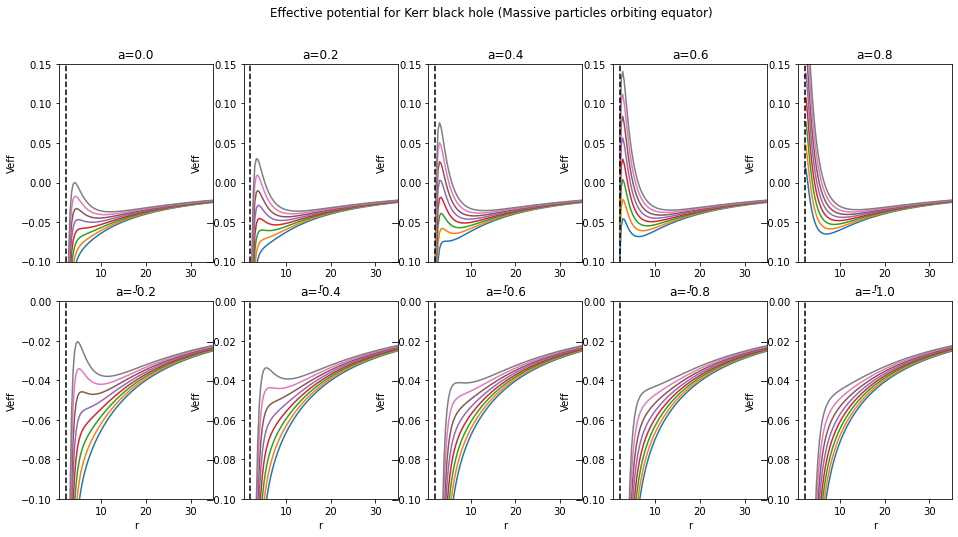
\includegraphics[width=\textwidth]{images/massive_particle_kerr_equator.png}
    \caption{Kerr BH massive particle potential around equator. Clearly all unstable, in contrast to massive orbit potentials.}
    \label{fig:Kerr BH massive particle potential around equator}
\end{figure}


\begin{figure}
    \centering
    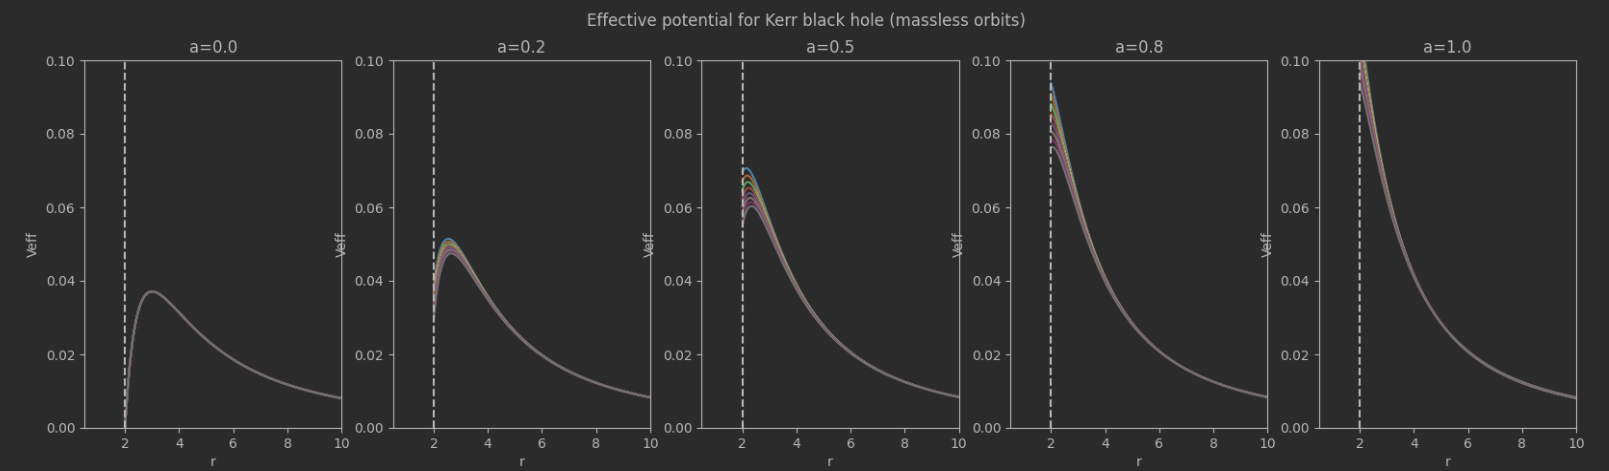
\includegraphics[width=\textwidth]{images/kerr massless orbit potential.png}
    \caption{Potential for massless particle orbits, around Kerr black hole}
    \label{fig:Kerr massless potential}
\end{figure}

See schwarzschild\_orbits.nb for more exploration.


Most Kerr black holes will be approaching the a=M ($J=M^2$) spin limit of the Kerr black hole, as angular momentum from accreting matter increases spin of BH. So in our diagram, a=1 is of most interest.

\section{Physical relevance of equations}

The equations that we have discussed produce non-physical situations when parameters reach certain values. We need to determine the validity range of all the parameters in the model, otherwise the model will produce garbage. These include hard boundaries, (no energy creation), and soft boundaries (particles have real mass).

\subsection{Hard boundaries}
\subsubsection{Schwarzschild black hole}

The four momentum can become imaginary for certain parameter values.To see one example of this, consider a radially infalling particle of mass $m>0$ in Schwarzschild spacetime. Can show (done in notebook - 24/03/2023) that for 

\begin{equation}
    v^2 = 1- \left( \frac{E^}{1-\frac{2M}{r}} \right) 
\end{equation}

This equation implies velocity becomes imaginary when 

\begin{equation}
    r < \frac{2M}{1-E}
\end{equation}

For a massless particle in the equatorial plane, it is shown in notebook, 

\begin{equation}
    \frac{dr}{dt} = -\left(1-\frac{2M}{r} \right) \sqrt{1-\frac{b^2}{r^2} \left(1-\frac{2M}{r}\right)}
\end{equation}

This expression becomes imaginary if

\begin{equation}
    b > \frac{r}{\sqrt{1-\frac{2m}{r}}}
\end{equation}

This can be inverted to find the allowable radius, see notebook (it is a pretty ugly solution to a cubic equation).

Interestingly, using the four momentum conservation equation (\ref{eq:sigma conservation}) for massless particles, the range where $\frac{dr}{d\tau}$ becomes imaginary only exists if the condition $b = 3\sqrt{3}GM$ is satisfied, i.e. if the particle is not bounded by the black hole. 

\subsubsection{Kerr black hole - soft boundaries}

For a particle with no angular momentum ($l=0$) and initial energy $e=1$ the shape of the orbit can be determined from equations (\ref{eq:Kerr dtdtau}) and (\ref{eq:Kerr dphidtau}), giving

\begin{equation}
    \frac{d\phi}{dr} = -\frac{2 M a}{r \Delta} \left[   \frac{2M}{r} \left(  1-\frac{a^2}{r^2}   \right)    \right]
\end{equation}\label{eq:Kerr radial inspiral}

For equation (\ref{eq:Kerr radial inspiral}) to yield real values, we must have $r>a=J/M$.

Note also, from the discussion in section (\ref{sec:Event horizons}, coordinate singularities occur when $\rho=0$ or $\Delta = 0$. The $\rho=0$ singularity occurs if

\begin{equation}
    r^2+a^2 \cos{\theta} = 0
    \Rightarrow
    \theta=\cos^{-1}{\left(-\frac{r^2}{a^2}\right)}
\end{equation}

This singularity indeed occurs, since $r \leq a$. The singularity corresponding to $\Delta=0$ occurs if

\begin{equation}
    r^2-2Mr+a^2=0
    \Rightarrow
    (r-M)^2+(a^2-M^2)=0
    
    \Rightarrow
    r=M\pm\sqrt{M^2-a^2}\label{eq:Kerr event horizon}
\end{equation}

Hence, we require $a<M\Rightarrow J < M^2$, i.e. the spin of the Kerr black hole is limited.


\section{Soft boundaries}

Penrose process? Blandford-Znajek mechanism? They aren't producing energy from nothing though.



\section{Double Schwarzschild}


\section{Astrophysical significance}\label{sec:Astrophysical significance}

The ISCO for massive particles will result in many particles orbiting the BH in this region. Interactions between the particles, resulting in energy transfer will result in particles accreting into the BH. The gravitational binding energy of the particles as they fall onto the BH will be released in the form of electromagnetic radiation, probably high energy x-rays, which can be observed.

In the case of Kerr black holes, the angular momentum of the accreting matter will be transferred to the BH, resulting in an increase in spin - this will push the BH to reach the maximal spin $J=M^2$.

The circular photon orbits correspond to the photon ring around the BH.The fact that the orbits are unstable means that photons will not stay in orbit forever, and will thus escape the black whole, resulting in a faintly visible ring.

The fact that orbits 


\section{GR and EM analogy}

Blandford-Znajek mechanism

Gravito-magnetism

Magnetic re-connection and sunspots

\subsection{Magnetic reconnection}

When magnetic field lines pointing in opposite directions cross, changing magnetic topology, releasing lots of energy 

\section{Appendix}

\subsection{Geometric units}

Throughout most of this document we will be using geometric units

\begin{equation}
    G = c = 1 \left(=M\right)
\end{equation}

If we have M represent the mass of the sun, then we get the following SI unit relations

\begin{align*}
    1kg &= \frac{1}{1.989 \cdot 10^{30}} \\
    1m &= \frac{1}{1477} \\
    1s &= 2.030 \cdot 10^5
\end{align*}



    

% \subsection{Lie derivatives and Killing vectors}


\bibliographystyle{unsrt}
\bibliography{sample}

\end{document}